\documentclass[aspectratio=169,11pt]{beamer}

\usetheme{Madrid}
\usecolortheme{default}
\usefonttheme{professionalfonts}
\setbeamertemplate{navigation symbols}{}
\setbeamertemplate{footline}[frame number]

\usepackage{amsmath, amssymb, booktabs, graphicx}
\graphicspath{{../../assets/figures/}{assets/figures/}}

\title{Mobility, Migration, and Intergenerational Transmission}
\subtitle{Labor I --- Week 10}
\author{Teaching deck draft}
\date{}

\begin{document}

\begin{frame}
  \titlepage
\end{frame}

\begin{frame}{Central question and motivation}
\begin{itemize}
    \item Week 10 asks how workers move across employers, occupations, places, and generations.
    \item Mobility is both an adjustment margin and a margin constrained by frictions.
    \item The labor question is whether movement changes access to better wage ladders, firms, and local opportunities.
\end{itemize}
\end{frame}

\begin{frame}{Bridge from Week 9}
\begin{itemize}
    \item Week 9 showed that opportunity sets may already be segmented by identity, firms, and places.
    \item Week 10 asks how workers move through that segmented architecture, and who remains stuck.
    \item This is the bridge from static inequality and discrimination to dynamic reallocation and persistence.
\end{itemize}
\end{frame}

\begin{frame}{Mobility objects and measurement}
\[
P_{jk} = \Pr(Q_{i,t+1}=k \mid Q_{it}=j, M_{it}=1),
\qquad
h_{it} = \Pr(M_{it}=1 \mid X_{it}, Z_t)
\]

\begin{itemize}
    \item Transition matrices tell us where movers go.
    \item Hazard rates tell us who moves and when.
    \item Employer, occupation, place, and intergenerational mobility are different objects.
\end{itemize}
\end{frame}

\begin{frame}{Transition matrix intuition}
\begin{center}
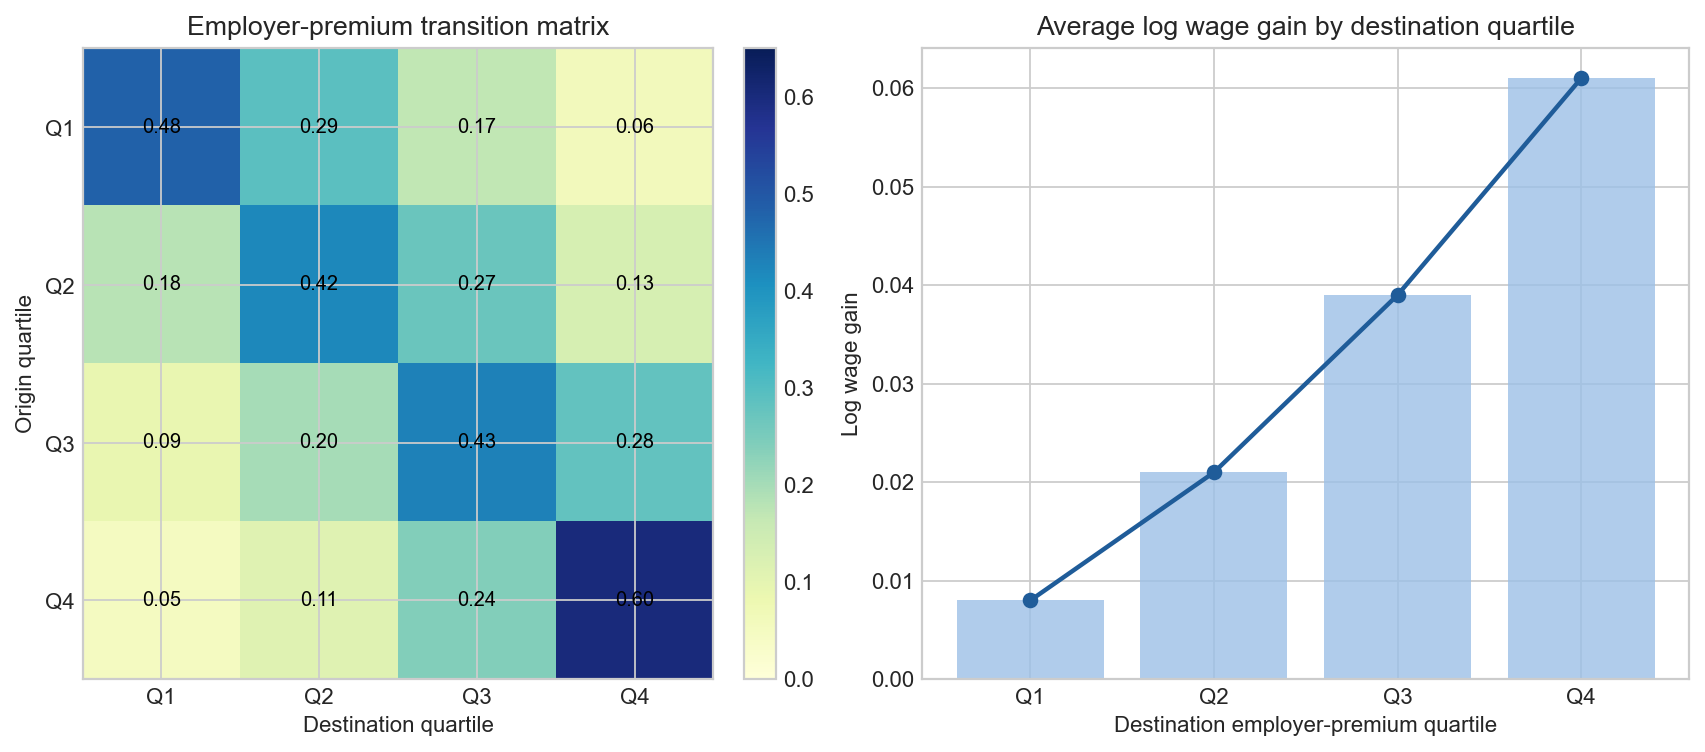
\includegraphics[height=0.72\textheight,keepaspectratio]{10-employer-mobility-transition-heatmap.png}
\end{center}
\end{frame}

\begin{frame}{Worker mobility and wage growth}
\[
\Delta \log w_{i,t+1} = \alpha + \beta M_{it}
+ \gamma \big(\psi_{f_{i,t+1}} - \psi_{f_{it}}\big) + \varepsilon_{it}
\]

\begin{itemize}
    \item Linked employer-employee data let us see whether wage growth comes from destination firms.
    \item Mobility is not neutral churn when firms sit on different wage ladders.
    \item Measurement correction matters because employer-to-employer flows are easy to undercount.
\end{itemize}
\end{frame}

\begin{frame}{Measurement correction for EE mobility}
\begin{center}
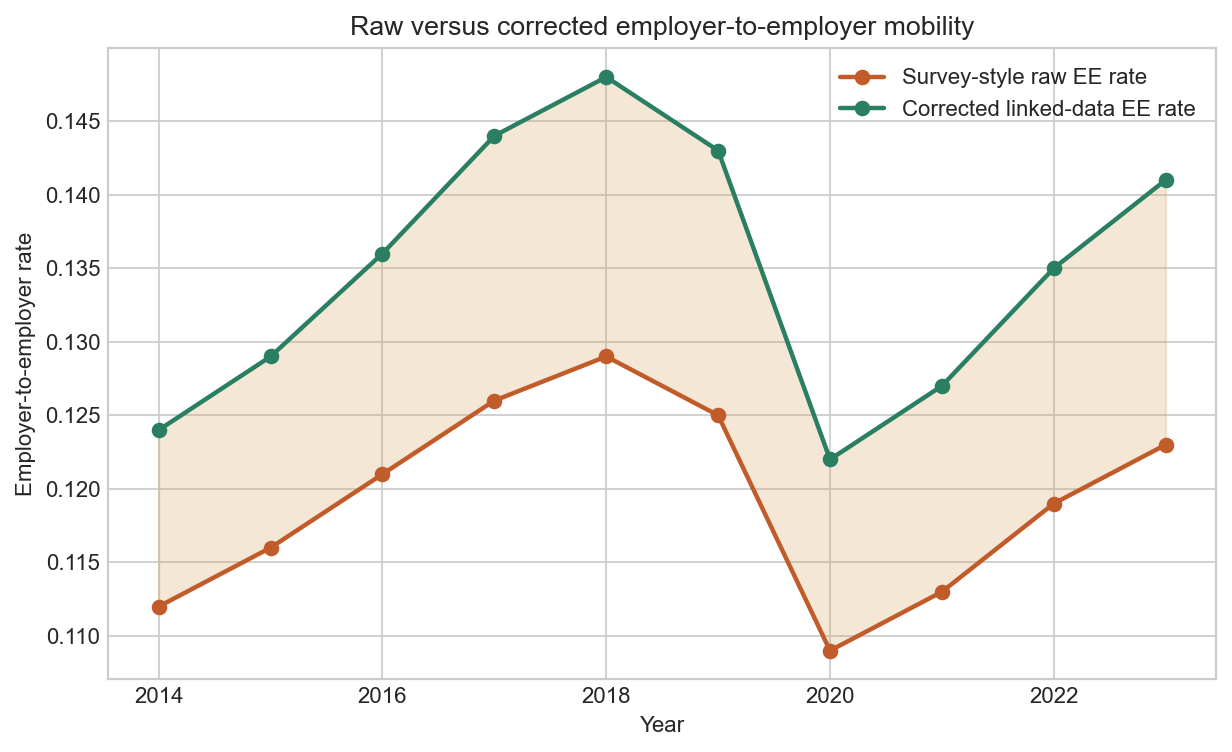
\includegraphics[height=0.72\textheight,keepaspectratio]{10-employer-mobility-measurement-correction.png}
\end{center}
\end{frame}

\begin{frame}{Migration as labor-market reallocation}
\[
M_i = \mathbf{1}\left\{
\max_{d \in \mathcal{D}} \big(\mu_d + r_d s_i + a_{id}\big)
- \big(\mu_o + r_o s_i + a_{io}\big)
- \kappa_{iod} > 0
\right\}
\]

\begin{itemize}
    \item Migration is an investment problem with selection.
    \item Returns depend on destination wage levels, returns to skill, and moving costs.
    \item Observed mover gains are not automatically causal because movers are selected.
\end{itemize}
\end{frame}

\begin{frame}{Roy-style migration selection}
\begin{center}
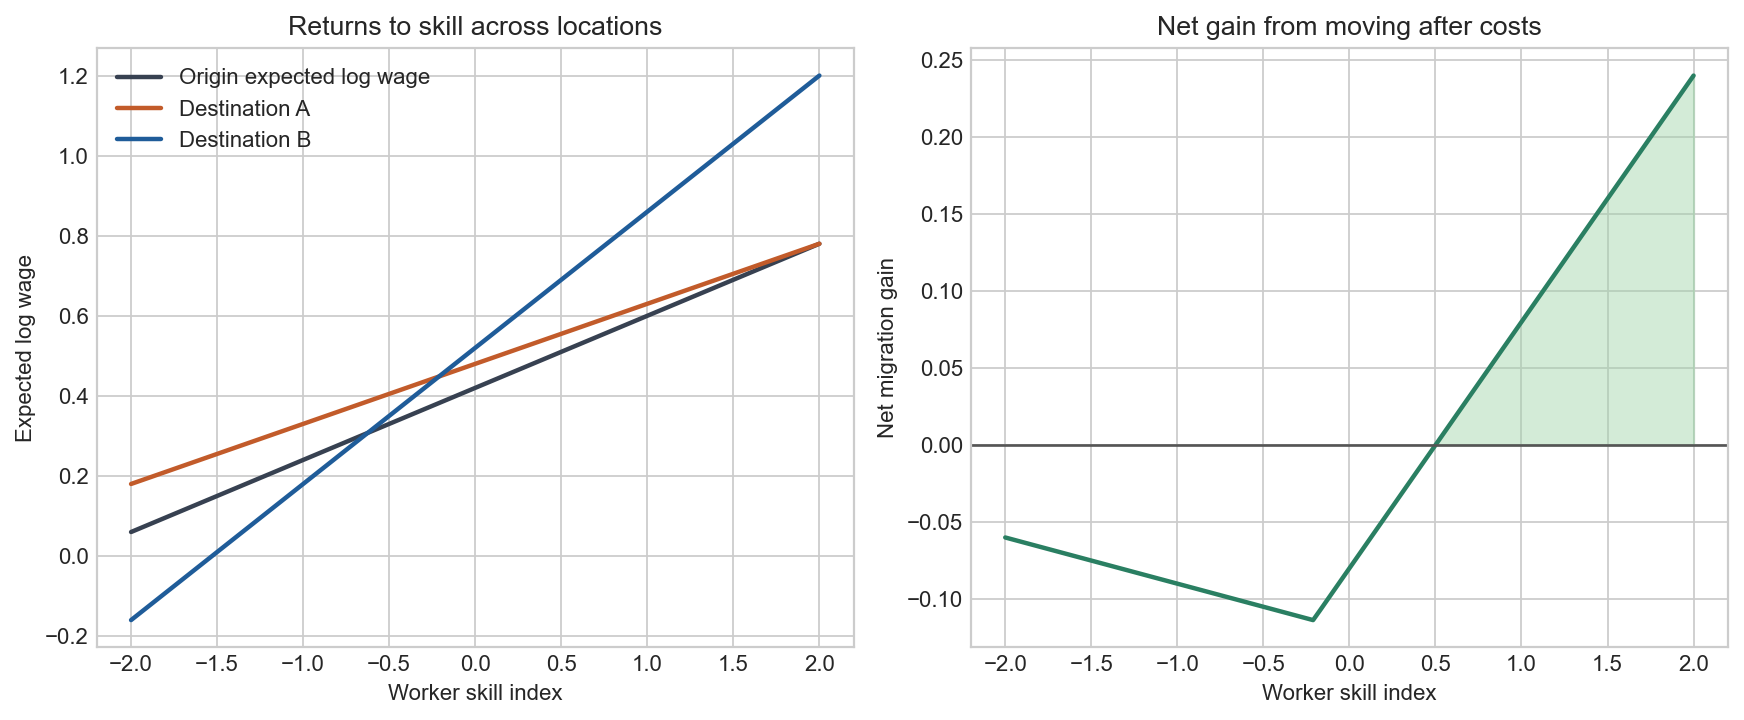
\includegraphics[height=0.72\textheight,keepaspectratio]{10-migration-selection-schematic.png}
\end{center}
\end{frame}

\begin{frame}{Credit, information, and moving frictions}
\[
\tau^{move} = \mathbb{E}[M_i(1) - M_i(0)]
\]

\begin{itemize}
    \item Credit lotteries identify what happens when one mobility friction is relaxed.
    \item This is different from comparing movers with stayers in observational data.
    \item The labor payoff can appear in distant moves, employer changes, or occupational upgrading.
\end{itemize}
\end{frame}

\begin{frame}{Migration reforms and exposure designs}
\[
Y_{rt} = \alpha_r + \delta_t + \beta (\text{Exposure}_r \times \text{Post}_t) + X_{rt}'\Gamma + \varepsilon_{rt}
\]

\begin{itemize}
    \item Reform and border designs ask how labor markets respond when migration access changes.
    \item The identifying variation is differential exposure to the reform, not raw migrant shares.
    \item These are reduced-form local-equilibrium effects, not one pure structural channel.
\end{itemize}
\end{frame}

\begin{frame}{Intergenerational transmission of labor outcomes}
\[
R_i^{child} = \alpha + \beta R_i^{parent} + u_i
\]

\begin{itemize}
    \item Rank-rank slopes summarize relative mobility across generations.
    \item Parent-child linked data reveal persistence across places, cohorts, and family backgrounds.
    \item The next question is which channels carry the persistence: skills, occupations, firms, or places.
\end{itemize}
\end{frame}

\begin{frame}{Rank-rank and mediation intuition}
\begin{center}
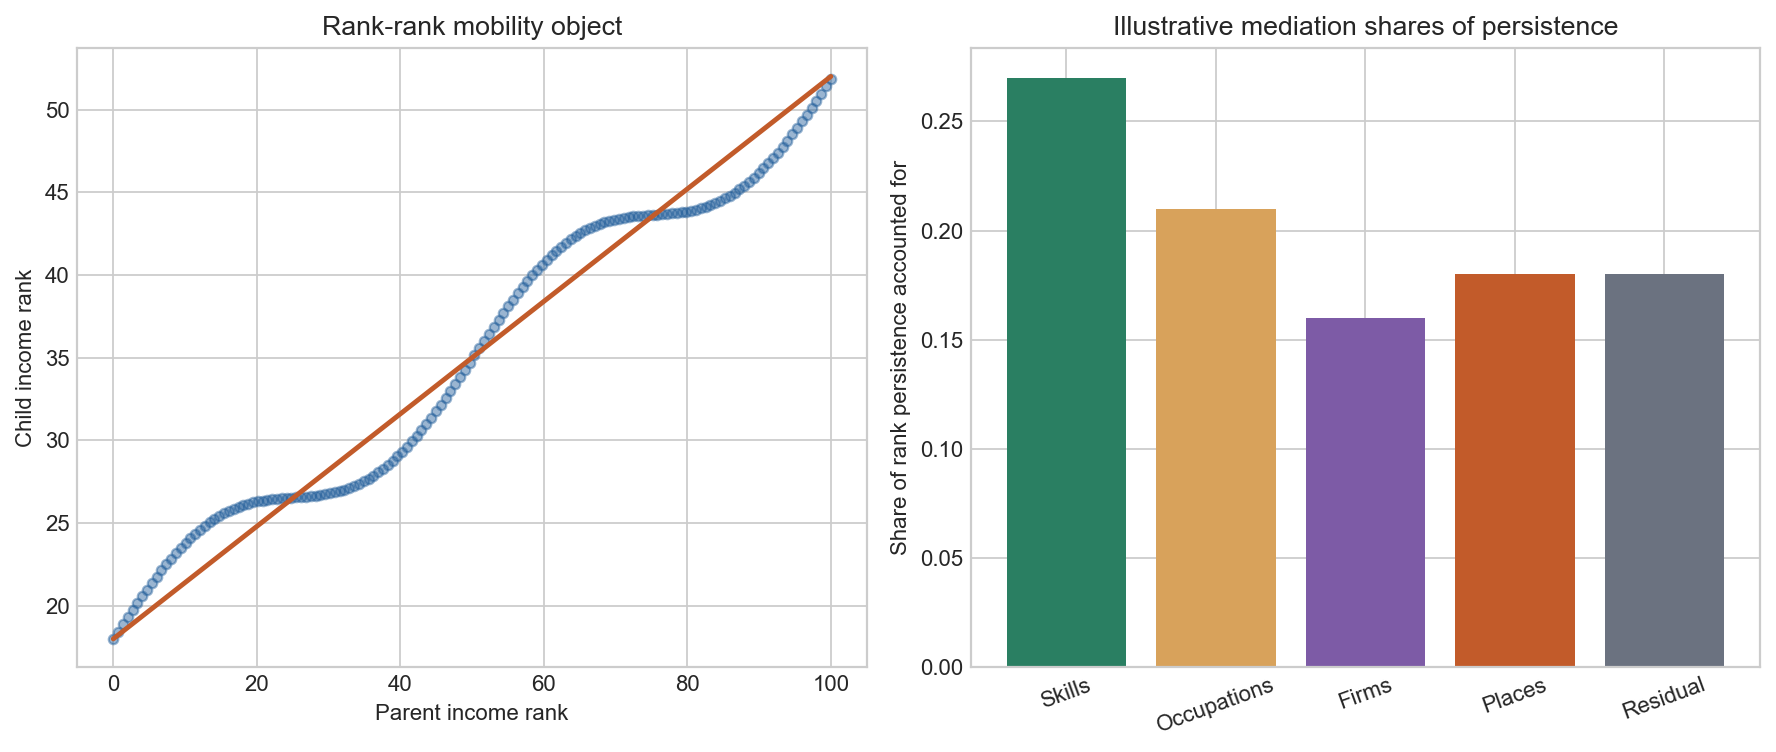
\includegraphics[height=0.72\textheight,keepaspectratio]{10-rank-rank-transmission-schematic.png}
\end{center}
\end{frame}

\begin{frame}{Empirical progress and causal designs}
\begin{itemize}
    \item Linked employer-employee data turned mobility into a firm-sorting question.
    \item Linked parent-child data turned mobility into a place and cohort mapping question.
    \item Lotteries, reforms, and exposure designs improved identification of frictions and migration shocks.
    \item Measurement correction improved the basic employer-to-employer mobility object itself.
\end{itemize}
\end{frame}

\begin{frame}{Inequality persistence through firms, occupations, and places}
\begin{itemize}
    \item Wage ladders differ across firms.
    \item Career ladders differ across occupations.
    \item Opportunity sets differ across places.
    \item Intergenerational persistence partly reflects differential access to those ladders.
\end{itemize}
\end{frame}

\begin{frame}{Bridge to Week 11 policy}
\begin{itemize}
    \item Week 11 asks which worker-side policies relax frictions or change incentives.
    \item Week 10 says policy targets may include liquidity, information, migration access, and place constraints.
    \item Mobility evidence helps decide whether the right intervention is cash, search help, training, or reform.
\end{itemize}
\end{frame}

\begin{frame}{Takeaways}
\begin{itemize}
    \item Mobility is a family of objects, not one statistic.
    \item Movement across firms, occupations, and places can amplify or reduce inequality persistence.
    \item Good mobility research combines better measurement with explicit identifying variation.
    \item Worker policy is partly about which mobility frictions are actually relaxable.
\end{itemize}
\end{frame}

\appendix

\begin{frame}{Appendix: optional extension block}
\begin{itemize}
    \item Careers and intergenerational mobility.
    \item Measurement correction for employer-to-employer reallocation.
    \item Housing, amenities, and place-based opportunity.
\end{itemize}
\end{frame}

\end{document}
